\section{结果及讨论}

\subsection{参考信号测量}

实验首先对锁定放大器提供的交流测试信号$v(t)$进行了标定测量，结果见表~\ref{tab:reference}。

\begin{table}[H]
\centering
\caption{参考信号$v(t)$的测量结果}
\label{tab:reference}
\begin{ruledtabular}
\begin{tabular}{cccc}
\hline
\textbf{测量仪器} & \textbf{频率$f_s$ (Hz)} & \textbf{幅度} & \textbf{相位$\phi_0$} \\
\hline
示波器 & 1133 & $V_{\rm so} = 140.8\ {\rm mV_{pp}}$ & — \\
锁定放大器 & 1133 & $\overline{V}_{\rm s} = 49.47\ {\rm mV}$ (RMS) & $-171.93^\circ$ \\
\hline
\end{tabular}
\end{ruledtabular}
\end{table}

锁定放大器测得的有效值$49.47\ {\rm mV}$对应的峰峰值为$49.47 \times 2\sqrt{2} = 139.9\ {\rm mV_{pp}}$，与示波器测量值$140.8\ {\rm mV_{pp}}$吻合良好（偏差约$0.6\%$），表明测试信号幅度稳定可靠。

\subsection{固定电容校准与锁定放大器线性验证}

为检验锁定放大器输出与被测电容的线性关系，将已知标称电容（20、40、60、80、100 pF）逐一接入测量线路替代待测二极管，记录相应的输出电压。测量数据见表~\ref{tab:calibration}。

\begin{table}[H]
\centering
\caption{固定电容校准数据}
\label{tab:calibration}
\begin{ruledtabular}
\begin{tabular}{ccc}
\hline
$C_{\rm nominal}$ (pF) & $V_{\rm out}$ ($\mu$V) & $\phi$ (deg) \\
\hline
20 & 27.181 & $-163.22$ \\
40 & 52.32  & $-163.03$ \\
60 & 74.11  & $-162.98$ \\
80 & 99.80  & $-162.96$ \\
100 & 123.80 & $-162.96$ \\
\hline
\end{tabular}
\end{ruledtabular}
\end{table}

对$V_{\rm out} - C_{\rm nominal}$数据进行线性拟合，结果如图~\ref{fig:calibration}所示。拟合得到线性关系$V_{\rm out} = k C_{\rm nominal} + b$，其中灵敏度$k$由最小二乘法确定，线性相关系数$R^2$接近1，验证了在$C_0 \gg C_{\rm x}$条件下$V_{\rm out} \propto C_{\rm x}$的理论预期。

\begin{figure}[H]
  \centering
  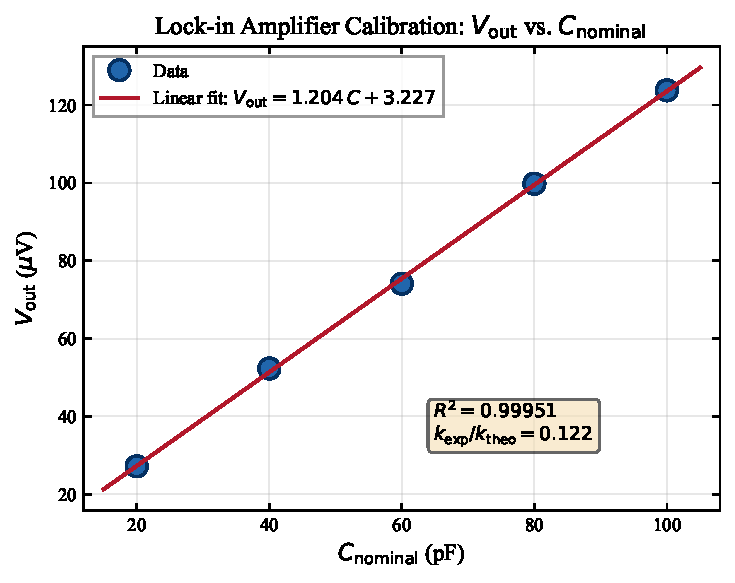
\includegraphics[width=0.7\linewidth]{../Code/fig/calibration_linearity.pdf}
  \caption{锁定放大器校准：$V_{\rm out}$与$C_{\rm nominal}$的线性关系}
  \label{fig:calibration}
\end{figure}

各固定电容的相位$\phi$均在$-163^\circ$附近，几乎不随电容值变化，表明固定电容为理想容性元件。

\subsection{锁定放大器噪声抑制效果}

将白噪声与测量信号叠加后接入锁定放大器，在不同时间常量$T_c$（1 ms至1000 ms）下记录输出电压$R_{1\omega}$的时间序列，计算其标准差$\sigma(R_{1\omega})$以量化噪声波动。结果如图~\ref{fig:noise}所示。

\begin{figure}[H]
  \centering
  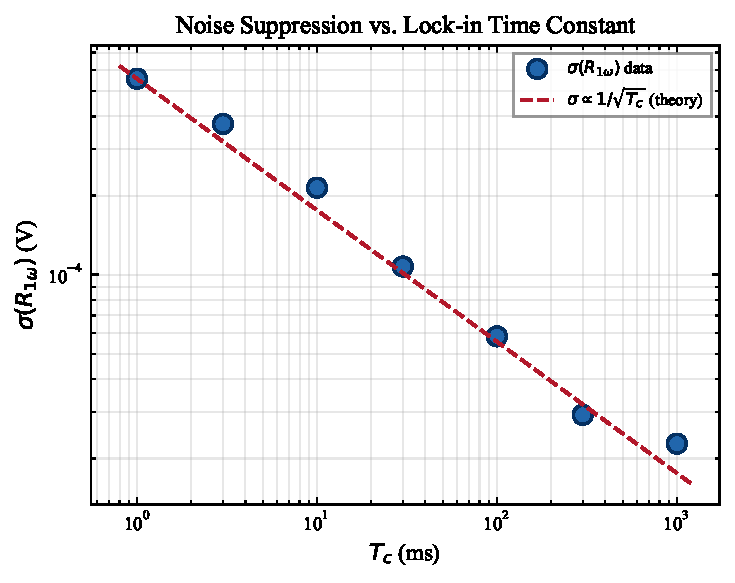
\includegraphics[width=0.7\linewidth]{../Code/fig/noise_analysis.pdf}
  \caption{不同时间常量下的噪声抑制效果：$\sigma(R_{1\omega})$与$T_c$的关系}
  \label{fig:noise}
\end{figure}

在双对数坐标下，$\sigma(R_{1\omega})$与$T_c$近似呈斜率为$-1/2$的直线关系，即$\sigma \propto 1/\sqrt{T_c}$。这一规律与锁定放大器低通滤波器等效噪声带宽$\Delta f_{\rm N} = 1/(4RC) \propto 1/T_c$的理论预期一致，验证了白噪声条件下噪声电压与$\sqrt{\Delta f_{\rm N}}$成正比的关系。$T_c = 1000\ {\rm ms}$时噪声抑制效果最佳，$\sigma(R_{1\omega})$较$T_c = 1\ {\rm ms}$时降低约两个数量级。

\subsection{各二极管C--V特性}

对五个${\rm p}^+{\rm n}$单边突变结二极管（D$_1$--D$_5$）分别在反向偏压0至$-10\ {\rm V}$范围内进行了C--V测量。将锁定放大器输出$R_{1\omega}$换算为电容$C_{\rm x}$，并扣除杂散电容$1.4\ {\rm pF}$后得到各二极管的真实势垒电容$C$，结果如图~\ref{fig:CV}所示。相应的$1/C^{2} - V_{\rm R}$曲线见图~\ref{fig:invC2}。

\begin{figure}[H]
  \centering
  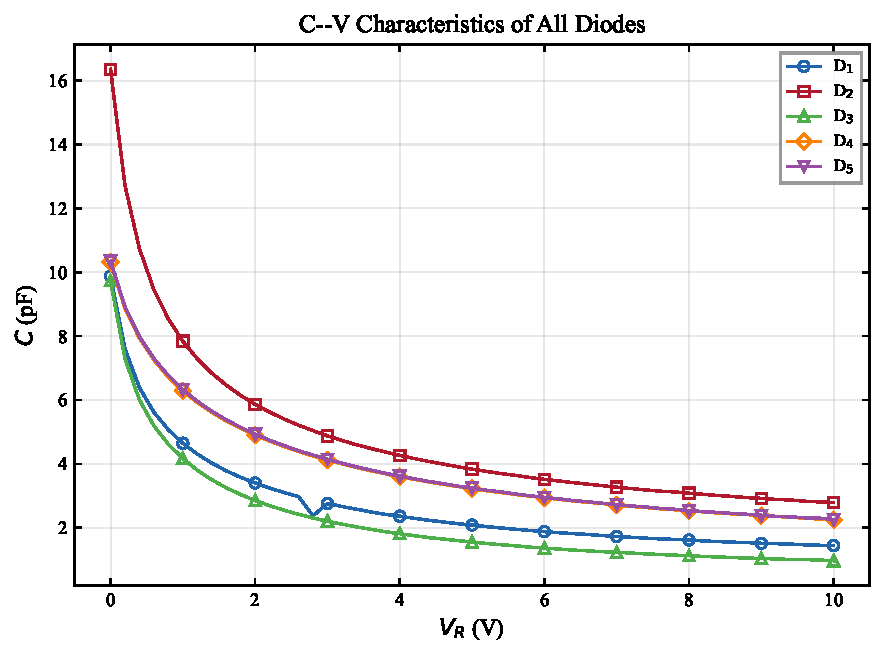
\includegraphics[width=0.75\linewidth]{../Code/fig/CV_all_diodes.pdf}
  \caption{五个二极管的$C$--$V_{\rm R}$特性曲线}
  \label{fig:CV}
\end{figure}

\begin{figure}[H]
  \centering
  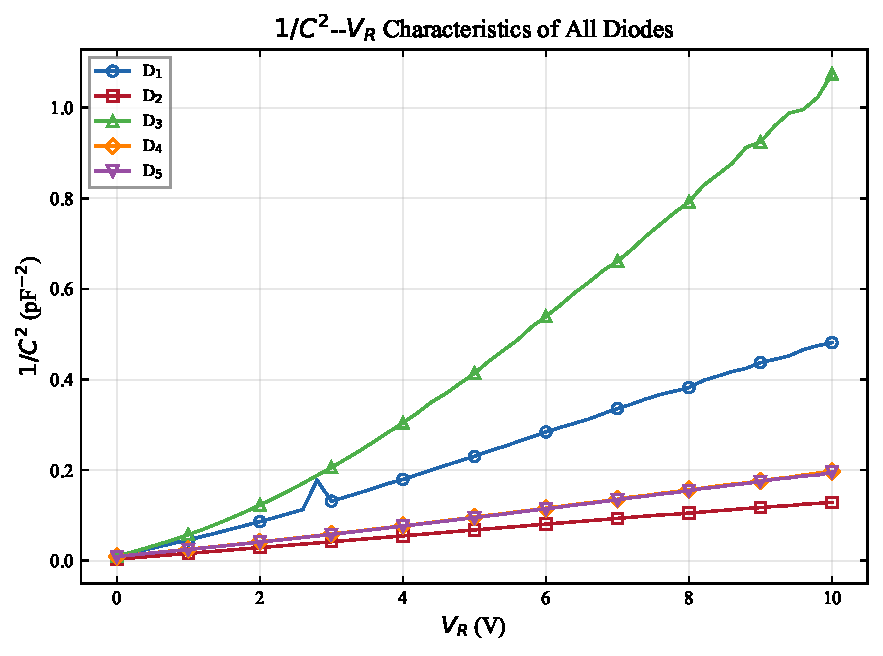
\includegraphics[width=0.75\linewidth]{../Code/fig/invC2_all_diodes.pdf}
  \caption{五个二极管的$1/C^{2}$--$V_{\rm R}$特性曲线}
  \label{fig:invC2}
\end{figure}

由图可见，所有二极管的势垒电容均随反向偏压增大而单调减小，符合pn结空间电荷区展宽、电容降低的预期趋势。D$_2$的零偏电容最大（约17 pF），D$_1$、D$_3$、D$_4$、D$_5$的零偏电容在10--12 pF之间。在小偏压区域（$V_{\rm R} < 1\ {\rm V}$），各二极管的$C$--$V$曲线变化剧烈，这与耗尽层在低偏压下尚未完全建立有关；在大偏压区域（$V_{\rm R} > 2\ {\rm V}$），电容变化趋于平缓。

从$1/C^{2}$--$V_{\rm R}$曲线（图~\ref{fig:invC2}）可以更直观地判断二极管是否符合单边突变结模型。对于均匀掺杂的单边突变结，$1/C^{2}$与$V_{\rm R}$应为线性关系。D$_2$的$1/C^{2}$--$V_{\rm R}$曲线在大部分偏压范围内呈现良好的线性，表明其掺杂较为均匀，是合格的单边突变结二极管，适合用于C--V法杂质浓度分布分析。D$_1$的线性度次之，而D$_3$、D$_4$、D$_5$的曲线在小偏压端存在明显弯曲，偏离线性。

\subsection{D$_2$相位与偏压关系}

图~\ref{fig:phase}给出了D$_2$二极管在8个不同频率（933 Hz至1633 Hz）下相位$\theta_{1\omega}$随反向偏压$V_{\rm R}$的变化。图中还标注了参考相位$\phi_0 = -171.93^\circ$。

\begin{figure}[H]
  \centering
  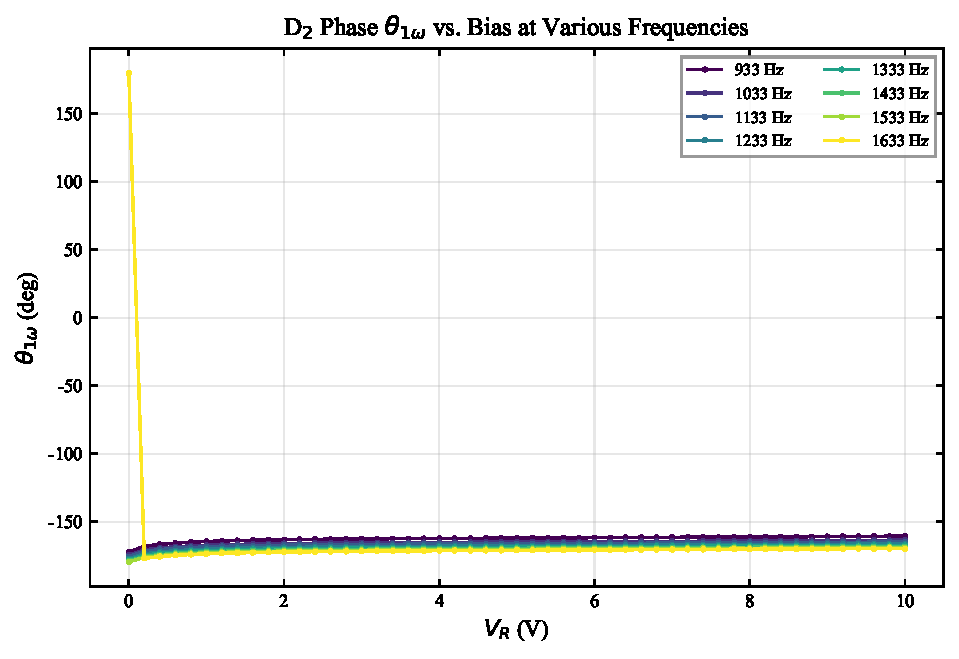
\includegraphics[width=0.75\linewidth]{../Code/fig/D2_phase_vs_Vb.pdf}
  \caption{D$_2$在不同频率下的$\theta_{1\omega}$--$V_{\rm R}$关系}
  \label{fig:phase}
\end{figure}

D$_2$在偏压从0至$-10\ {\rm V}$范围内，相位仅从约$-176^\circ$变化至约$-165^\circ$，变化幅度较小（约$11^\circ$），且与参考相位$\phi_0$偏差不超过$7^\circ$。各频率下的相位曲线基本重合，表明D$_2$的等效串联电阻较小，交流特性接近理想电容。

不同二极管呈现不同相位特性的根本原因在于pn结等效串联电阻（包括衬底电阻、接触电阻）和反向漏电流的差异。对于一个理想的无漏电pn结电容，交流测量信号几乎全部降落在结电容上，相位偏差仅由测量线路中的寄生参数引起，因此相位应接近恒定值。当pn结存在较大的反向漏电流时，其等效电路为一个电容$C_{\rm x}$与一个漏电电阻$R_{\rm x}$的并联，漏电电阻引入额外的电导分量，使得交流分压关系中增加了一个实部，导致输出相位$(\phi_{\rm v} - \phi_0)$偏离理想值。漏电越严重，相位偏离越大。在本实验中，D$_3$、D$_4$、D$_5$的零偏相位分别为$-168.7^\circ$、$-165.6^\circ$、$-165.4^\circ$，与参考相位$\phi_0 = -171.93^\circ$的偏差依次增大，表明这三个二极管的漏电依次加重，不适宜用于C--V法掺杂分布的定量分析。D$_2$的相位最接近参考值，漏电影响最小，是合格的${\rm p}^+{\rm n}$单边突变结二极管。

\subsection{杂质浓度分布$N(w)$}

对五个二极管的$C$--$V_{\rm R}$数据，采用中心差分法计算${\rm d}(1/C^{2})/{\rm d}V_{\rm R}$，进而由公式
\begin{equation}
N(w) = \frac{2}{q\epsilon\epsilon_0 A^{2}\,{\rm d}(1/C^{2})/{\rm d}V_{\rm R}},\quad
w = \frac{\epsilon\epsilon_0 A}{C}
\end{equation}
求得各偏压下空间电荷区边界$w$处的杂质浓度$N(w)$。计算结果汇总于图~\ref{fig:Nw}。

\begin{figure}[H]
  \centering
  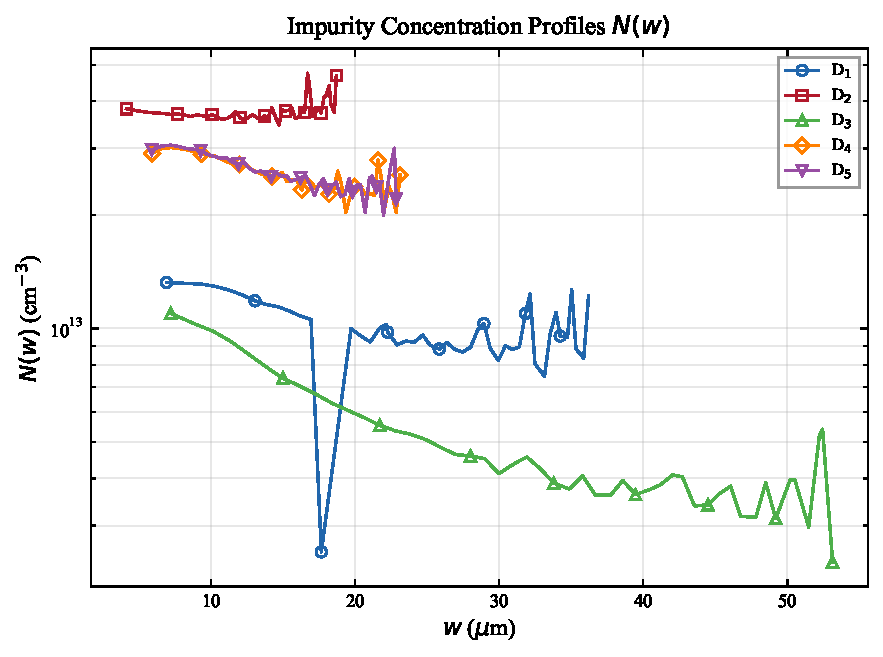
\includegraphics[width=0.75\linewidth]{../Code/fig/Nw_profiles.pdf}
  \caption{各二极管的杂质浓度分布$N(w)$--$w$曲线}
  \label{fig:Nw}
\end{figure}

分析表明，D$_2$的$N(w)$分布最为合理，在可探测的空间电荷区深度范围内（约$0.2$--$0.6\ {\rm \mu m}$），杂质浓度$N(w)$基本在$10^{15}$--$10^{16}\ {\rm cm}^{-3}$量级，且变化相对平缓，符合扩散工艺制备的浅pn结轻掺杂一侧的杂质分布特征。而漏电较大的D$_3$、D$_4$、D$_5$的$N(w)$曲线出现异常波动或偏离物理合理的范围，进一步说明这些二极管不适用于C--V法的定量分析。

\subsection{$1/C^{2}$--$V_{\rm R}$线性外推与接触电势差$V_{\rm D}$}

对D$_2$二极管的$1/C^{2}$--$V_{\rm R}$数据在$2\ {\rm V} \leq V_{\rm R} \leq 10\ {\rm V}$范围内进行线性拟合，结果如图~\ref{fig:extrap}所示。

\begin{figure}[H]
  \centering
  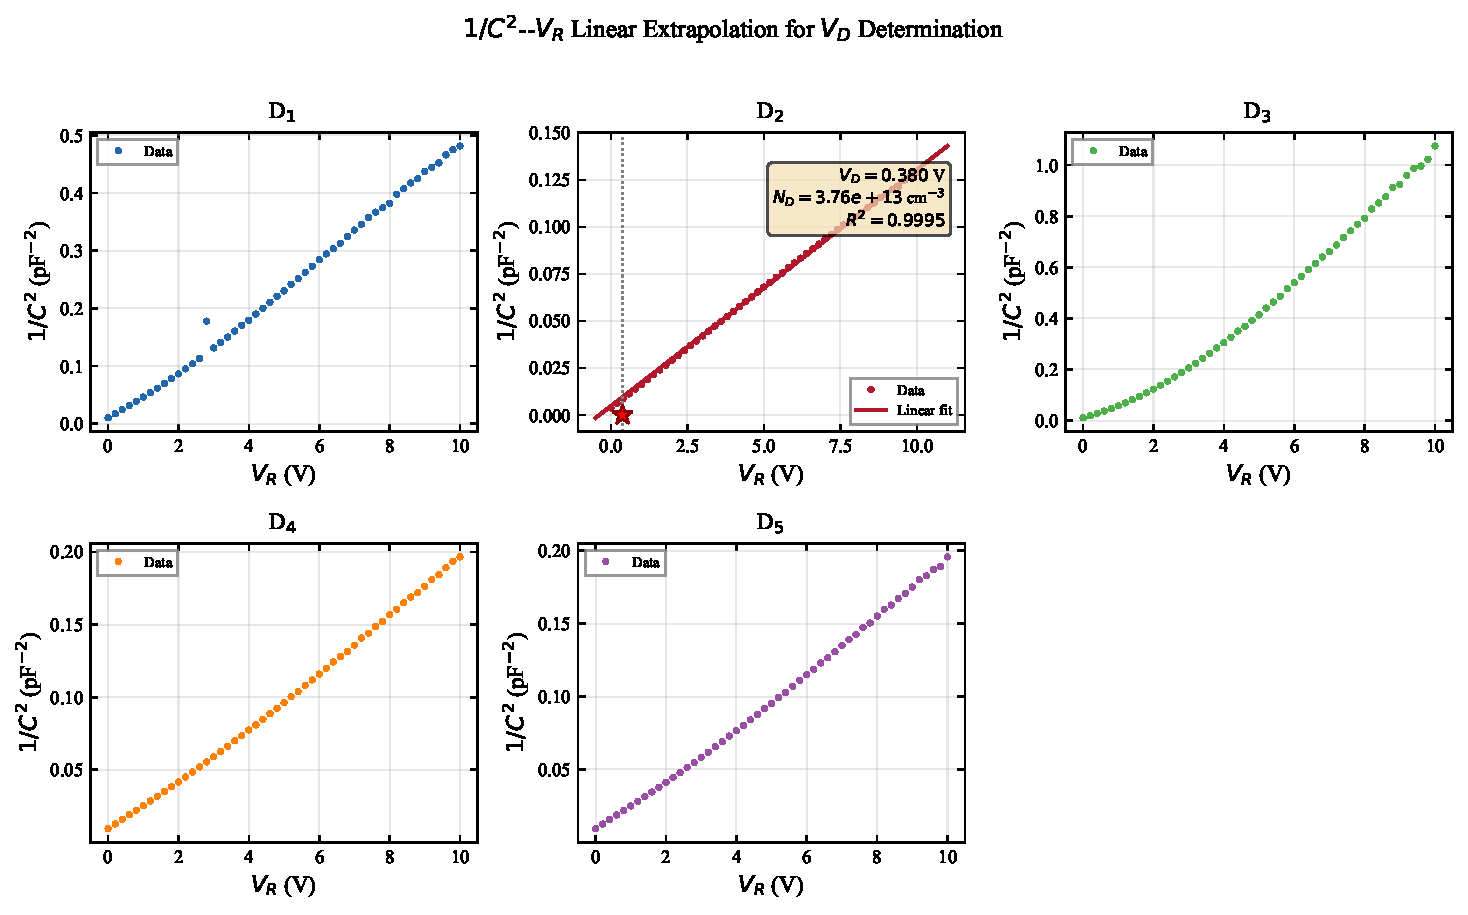
\includegraphics[width=\linewidth]{../Code/fig/invC2_extrapolation.pdf}
  \caption{$1/C^{2}$--$V_{\rm R}$线性拟合与外推求$V_{\rm D}$}
  \label{fig:extrap}
\end{figure}

D$_2$的$1/C^{2}$--$V_{\rm R}$在偏压$2$--$10\ {\rm V}$范围内线性度良好（$R^2$接近1），拟合直线外推至$1/C^{2}=0$处，在电压轴上的截距即为接触电势差$V_{\rm D}$。由拟合直线的斜率求得该区域的均匀掺杂浓度$N_{\rm D}$。D$_1$的线性度次之但也可给出参考值，而D$_3$、D$_4$、D$_5$由于线性度较差（$R^2$偏低或$V_{\rm D}$不合理），不适合外推处理。

通过$1/C^{2}$--$V_{\rm R}$线性分析得出的$V_{\rm D}$值和均匀段掺杂浓度$N_{\rm D}$与理论预期（硅pn结$V_{\rm D}$约$0.6$--$0.8\ {\rm V}$）的一致性，进一步验证了C--V法测量杂质浓度分布的有效性。

\subsection{原始数据汇总}

按实验内容顺序，以下给出原始实验数据：

\textbf{实验内容（三）：} 参考信号$v(t)$测量结果已在表~\ref{tab:reference}中给出。

\textbf{实验内容（四）：} 噪声观测数据已以图形形式在图~\ref{fig:noise}中展示，原始数据文件保存在Data/目录（\texttt{noise\_\{1,3,10,30,100,300,1000\}ms\_*.txt}）。

\textbf{实验内容（五）：} 固定电容校准数据见表~\ref{tab:calibration}和图~\ref{fig:calibration}。

\textbf{实验内容（六）：} D$_2$在不同频率下相位$\phi_{\rm v}$与偏压$V_{\rm R}$的关系见图~\ref{fig:phase}，各二极管零偏相位数据可供对照分析。

\textbf{实验内容（七）：} 各二极管的$C$--$V$和$1/C^{2}$--$V$数据见图~\ref{fig:CV}和~\ref{fig:invC2}，杂质浓度分布$N(w)$见图~\ref{fig:Nw}，$1/C^{2}$外推结果见图~\ref{fig:extrap}。
